\chapter{A Framework for SV Detection in MapReduce}\label{chap_framework}

\section{MapReduce Constraints on SV Algorithms}

MapReduce~\cite{Dean:2008p277} divides computation across a cluster into three phases. In the first phase, \emph{mappers} developed by the application programmer examine small blocks of data and emit a set of $\langle key, value \rangle$ pairs for each block examined. The MapReduce framework then sorts the output of the mappers by key, and aggregates all values that are associated with each key. Finally, the framework executes \emph{reducers}, also created by the application developer, which process all of the values for a particular key and produce one or more outputs that summarize or aggregate those values. MapReduce and Hadoop allow efficient processing of large data sets by scheduling tasks for execution as close as possible to the nodes which hold the required data, minimizing network traffic and I/O contention.

The need to separate logic into mappers and reducers makes it difficult to implement traditional RP-based SV detection approaches in MapReduce, particularly given the global clustering of paired end mappings at the heart of many RP approaches. MapReduce algorithms, by contrast, excel at conducting many independent calculations in parallel. The sequencing applications that have been implemented in MapReduce succeed by dividing processing into a series of local computation, for example calling a SNV at a particular location in the genome given the reads that cover it, which is the approach taken by the variant callers GATK~\cite{McKenna:2010p1051} and Crossbow~\cite{Langmead:2009p1225}. SV approaches that are similarly based on local computations have been described: the RP-based SV callers MoDIL~\cite{Lee:2009da} and forestSV~\cite{Michaelson:2012fj} try to solve the SV detection problem by computing scores or features along the genome and then producing SV predictions from those features in a post-processing step. 

\section{A General MapReduce SV Detection Algorithm}\label{section_general_algo}

Using this strategy, we have developed a conceptual algorithmic framework for SV detection in MapReduce, which is outlined in Algorithm~\ref{cb_algo}. This framework divides processing into three separate MapReduce jobs: an alignment job, a feature computation job, and an SV calling job. The overall workflow of the algorithm and its implementation on a compute cluster or cloud is summarized in Figure~\ref{cloudbreak_workflow}.

\begin{figure}
\centering
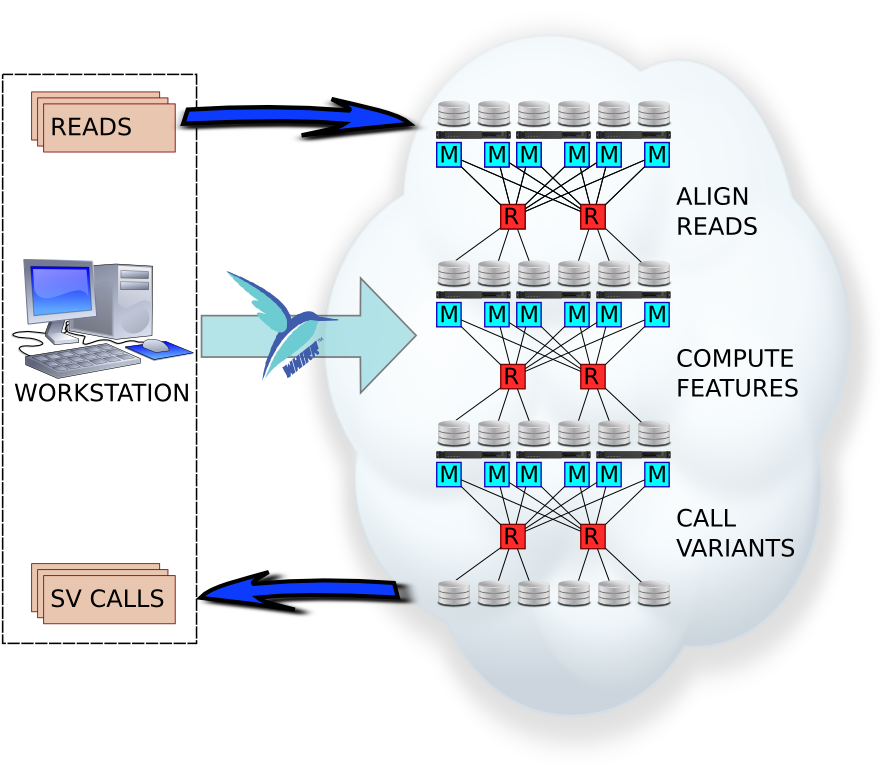
\includegraphics[width=.8\textwidth]{figures/workflow_with_whirr.png}
\caption{An overview of the steps of the MapReduce SV detection workflow. Reads are first uploaded to a Hadoop cluster from local storage. Processing is then then divided into three MapReduce jobs: 1) Mapping with sensitive settings. 2) Computation of features across the genome. 3) Calling structural variations based on the features computed in the previous step. Finally, SV predictions can be downloaded from the Hadoop cluster and examined and annotated. Cloudbreak can also use the Apache Whirr library to automatically provision Hadoop clusters on and deploy data to cloud providers such as Amazon Elastic Compute Cloud.}
\label{cloudbreak_workflow}
\end{figure}


The \textsc{Align Reads} job uses existing alignment tools to discover mapping locations for each read pair. Aligners can be executed to report multiple possible mappings for each read, or only the best possible mapping. Given a set of read pairs, each of which consists of a read pair identifier $rpid$ and two sets of sequence and quality scores $<s,q>$, each mapper aligns each pair end set $<s,q>$ in either single- or paired end mode and emits possible mapping locations under the $rpid$ key. Reducers then collect the alignments for each paired end, making them available under one key for the next job. 

In the \textsc{Compute Features} job, we compute a set of features for each location in the genome. To begin, we tile the genome with small fixed-width, non-overlapping intervals. For the experiments reported in Chapter~\ref{chap_cloudbreak_eval} we use an interval size of 25bp (see Section~\ref{section_window_size} for an exploration of the effects of different window sizes on accuracy and runtime). Let $L = \left\{l_1,l_2,\ldots,l_N\right\}$ be the set of intervals covering the entire genome. Let $R^1 = \left\{r^{1}_{1},r^{1}_{2},\ldots,r^{1}_{M}\right\}$ and $R^2 = \left\{r^{2}_{1},r^{2}_{2},\ldots,r^{2}_{M}\right\}$ be the input set of paired reads. Let $A^1 = \left\{a^{1}_{m,1},a^{1}_{m,2},\ldots,a^{1}_{m,K}\right\}$ and $A^2 = \left\{a^{2}_{m,1},a^{2}_{m,2},\ldots,a^{2}_{m,L}\right\}$ be the set of alignments for the left and right reads from read pair $m$. For any given pair of alignments of the two reads in a read pair, $a^{1}_{m,i}$ and $a^{2}_{m,j}$, let the $\textrm{ReadPairInfo } rpi_{m,i,j}$ be information about the pair relevant to detecting SVs, e.g. the fragment size implied by the alignments and the likelihood that the alignments are correct. We then leave two functions to be implemented depending on the application:
\begin{flalign*}
 \textsc{Loci } :& \langle a^{1}_{m,i},a^{2}_{m,j} \rangle \rightarrow L_m \subseteq L \\
 \Phi :& \left\{\textrm{ReadPairInfo }rpi_{m,i,j}\right\} \rightarrow \mathbb{R}^N \\
\end{flalign*}

The first function, \textsc{Loci}, maps an alignment pair to a set of genomic locations to which it is relevant for SV detection; for example, the set of locations overlapped by the internal insert implied by the read alignments.  We optimize this step by assuming that if there exist concordant mappings for a read pair, defined as those where the two alignments are in the proper orientation and with an insert size within three standard deviations of the expected library insert size, one of them is likely to be correct and therefore we do not consider any discordant alignments of the pair. The second function, $\Phi$, maps a set of ReadPairInfos relevant to a given location to a set of real-valued vectors of features useful for SV detection. 

Finally, the third MapReduce job, \textsc{Call Variants}, is responsible for making SV calls based on the features computed at each genomic location. It calls another application-specific function: 

 \[ \textsc{PostProcess} : \left\{\phi_1,\phi_2,\ldots,\phi_N\right\} \rightarrow \left\{\langle  \textrm{SVType } s, l_{start}, l_{end} \rangle\right\} \]

This function maps the sets of features for related loci into a set of SV calls characterized by their type $s$ (i.e Deletion, Insertion, etc.) and their breakpoint locations $l_{start}$ and $l_{end}$. We parallelize this job in MapReduce by making calls for each chromosome in parallel, which we achieve by associating a location and its set of features to its chromosome in the map phase, and then making SV calls for one chromosome in each reduce task.

\begin{algorithm}
\algrenewcommand\algorithmicprocedure{\textbf{job}}
 \begin{algorithmic}[1]
 \Procedure{Alignment}{}
 \Function{Map}{$\textrm{ReadPairId }rpid, \textrm{ReadId }r, \textrm{ReadSequence }s, \textrm{ReadQuality }q$}
 \ForAll{$ \textrm{Alignments }a \in \textsc{Align}(<s,q>)$}
 \State $\textsc{Emit}(\textrm{ReadPairId }rpid, \textrm{Alignment }a)$
 \EndFor
 \EndFunction
 \Function{Reduce}{$\textrm{ReadPairId }rpid, \textrm{Alignments }a_{1,2,\ldots}$}
 \State $\textrm{AlignmentPairList }ap \gets \textsc{ValidAlignmentPairs}(a_{1,2,\ldots})$
 \State $\textsc{Emit}(\textrm{ReadPairId }rp, \textrm{AlignmentPairList } ap)$
 \EndFunction
 \EndProcedure

 \Procedure{Compute SV Features}{}
 \Function{Map}{$\textrm{ReadPairId }rp, \textrm{AlignmentPairList }ap$}
 \ForAll{$ \textrm{AlignmentPairs }<a_1,a_2> \in ap$}
 \ForAll{$ \textrm{GenomicLocations }l \in \textsc{Loci }(a_1,a_2)$}
 \State $ \textrm{ReadPairInfo }rpi \gets <\textrm{InsertSize}(a_1,a_2), \textrm{AlignmentScore}(a_1,a_2)>$
 \State $\textsc{Emit}(\textrm{GenomicLocation }l, \textrm{ReadPairInfo }rpi)$
 \EndFor
 \EndFor
 \EndFunction
 \Function{Reduce}{$\textrm{GenomicLocation }l, \textrm{ReadPairInfos }rpi_{1,2,\ldots}$}
 \State $\textrm{SVFeatures } \phi_l \gets \Phi(\textrm{InsertSizes }i_{1,2,\ldots}, \textrm{AlignmentScores }q_{1,2,\ldots})$
 \State $\textsc{Emit}(\textrm{GenomicLocation }l, \textrm{SVFeatures } \phi_l)$
 \EndFunction
 \EndProcedure

 \Procedure{Call SVs}{}
 \Function{Map}{$\textrm{GenomicLocation }l, \textrm{SVFeatures } \phi_l$}
 \State $\textsc{Emit}(\textrm{Chromosome}(l), <l,\phi_l>)$
 \EndFunction
 \Function{Reduce}{$\textrm{Chromosome }c, \textrm{GenomicLocation } l_{1,2,\ldots},\phi_{1,2,\ldots}$}
 \State $\textrm{StructuralVariationCalls } svs_c \gets \textsc{PostProcess }(\phi_{1,2,\ldots})$
 \EndFunction
 \EndProcedure
 \end{algorithmic}
\caption{The algorithmic framework for SV calling in MapReduce.}
\label{cb_algo}
\end{algorithm}

\section{Discussion}

